%!TeX spellcheck = fr-FR
\documentclass[10pt,fleqn]{article} % Default font size and left-justified equations
\usepackage[%
    pdftitle={SLCI : Transformée de Laplace},
    pdfauthor={Xavier Pessoles}]{hyperref}

\usepackage{import}
\usepackage{subcaption}
\subimport{../../../../style/}{preambule.tex}
%\fichetrue
\fichefalse
\proftrue
%\proffalse
%\tdtrue
\tdfalse
\courstrue
%\coursfalse
\subimport{../../../../style/}{new_style}
\subimport{../../../../style/}{macros_SII}
\subimport{../../../../style/}{preambule_trou.tex}

\usepackage{siunitx}
% -------------------------------------
% Déclaration des titres
% -------------------------------------

\def\discipline{Enseignement \\Technologique \\ Transversal}
\def\xxtete{Enseignement Technologique Transversal}

\def\classe{1 STI2D}
\def\xxnumpartie{Seq 3}
\def\xxpartie{Alimenter un système en énergie}

\def\xxnumchapitre{Séance 3}
\def\xxchapitre{\hspace{.12cm} Transmettre l'énergie}

\def\xxposongletx{2}
\def\xxposonglettext{1.45}
\def\xxposonglety{23}
\def\xxonglet{Seq. 3 -- Se. 6}

\def\xxactivite{Cours}
\def\xxauteur{\textsl{Geoffrey Vaquette}}

\def\xxcompetences{%
\textsl{%
\textbf{Prérequis :}
\begin{itemize}[label=\ding{112},font=\color{ocre}]
\item Analyse fonctionnelle de la chaîne d'énergie
\end{itemize}
\textbf{Savoirs et compétences :}
\begin{itemize}[label=\ding{112},font=\color{ocre}]
\item CO2.1	Identifier les flux et la forme de l'énergie, caractériser ses transformations et/ou modulations et estimer l'efficacité globale d'un système.
\end{itemize}
%
}}

\def\xxfigures{
\begin{center}
% 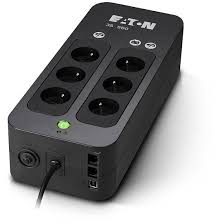
\includegraphics[width=2cm]{images/onduleur} \\
% 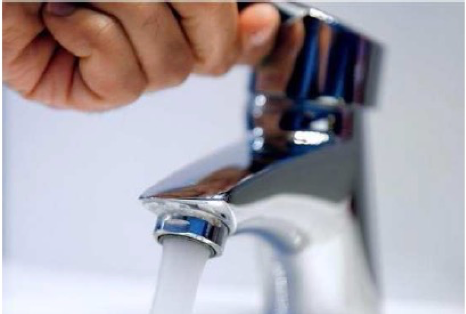
\includegraphics[width=2cm]{images/robinet} \\
%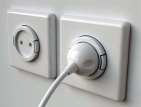
\includegraphics[width=2cm]{images/prise.png} \\
\end{center}
}%figues de la page de garde
\def\xxpied{%
Transmettre l'énergie \xxactivite%
}

%---------------------------------------------------------------------------
\renewcommand{\RemplirTrou}{false}
\begin{document}
\chapterimage{images/pignon_chaine.png}
\subimport{../../../../style/}{new_pagegarde}
\begin{figure}[h]
  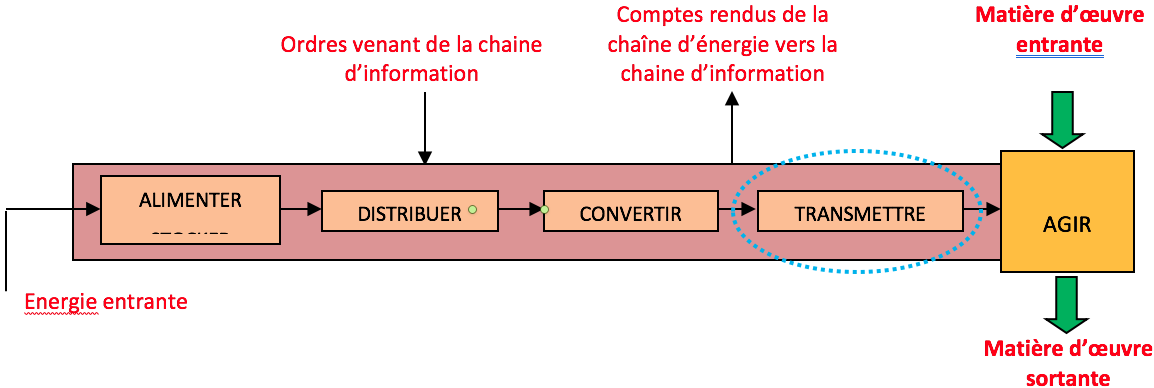
\includegraphics[width=\textwidth]{images/S03_C04}
  \caption{La fonction « Transmettre » dans la chaîne d'énergie}
  \label{fig:chaine}
\end{figure}

\section{Introduction}
\begin{aretenir}
  La fonction « Transmettre » permet
  \begin{itemize}
    \item D'adapter l’énergie du point de vue des efforts ou de la vitesse grâce aux réducteurs à engrenage, aux systèmes poulies-courroie ou pignons-chaîne
    \item De transformer l’énergie pour passer d’un type de mouvement à un autre type de mouvement. Par exemple, pour passer d’un mouvement de rotation à un mouvement de translation.
  \end{itemize}
\end{aretenir}
\begin{figure}[h]
  \centering
  \begin{subfigure}{0.25\textwidth}
    \centering
    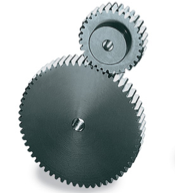
\includegraphics[width=0.9\textwidth,height=.1\textheight,keepaspectratio]{images/engr_droit}
    \caption{\trou{Engrenage droit}}
  \end{subfigure}\hfill
  \begin{subfigure}{.25\textwidth}
    \centering
    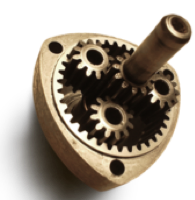
\includegraphics[width=0.9\textwidth,height=.1\textheight,keepaspectratio]{images/engr_epi}
    \caption{\trou{Train épicycloïdal}}
  \end{subfigure}\hfill
  \begin{subfigure}{0.25\textwidth}
    \centering
    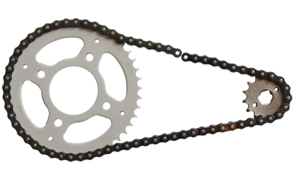
\includegraphics[width=0.9\textwidth,height=.1\textheight,keepaspectratio]{images/pignon_chaine}
    \caption{\trou{Pignon-chaîne}}
  \end{subfigure}\hfill
  \begin{subfigure}{.25\textwidth}
    \centering
    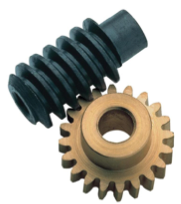
\includegraphics[width=0.9\textwidth,height=.1\textheight,keepaspectratio]{images/roue_vis}
    \caption{\trou{Roue vis sans fin}}
  \end{subfigure}\\
  \begin{subfigure}{0.25\textwidth}
    \centering
    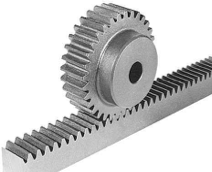
\includegraphics[width=0.9\textwidth,height=.1\textheight,keepaspectratio]{images/cremaillere}
    \caption{\trou{Crémaillère}}
  \end{subfigure}\hfill
  \begin{subfigure}{.25\textwidth}
    \centering
    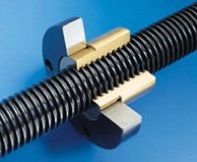
\includegraphics[width=0.9\textwidth,height=.1\textheight,keepaspectratio]{images/vis_ecrou}
    \caption{\trou{Vis-écrou}}
  \end{subfigure}\hfill
  \begin{subfigure}{0.25\textwidth}
    \centering
    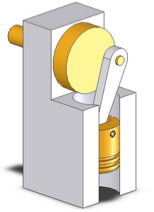
\includegraphics[width=0.9\textwidth,height=.1\textheight,keepaspectratio]{images/bielle_manivelle}
    \caption{Bielle-manivelle}
  \end{subfigure}
  \caption{Quelques exemples d'éléments de la fonction « Transmettre »}
  \label{fig:exemples}
\end{figure}

\section{Transmission de puissance par engrenages}
\begin{definition}
  Un engrenage est un système mécanique composé de deux roues dentées qui se transmettent la puissance par obstacle.
  Si un système de transmission par roues dentées est composé de plus de 2 roues alors c’est ce système est un train d’engrenages.
\end{definition}

\begin{remark}
  a roue la plus petite d’un engrenage est appelée un \trou{pignon}.
\end{remark}

Les engrenages sont utilisés dans toutes les branches de la mécanique pour transmettre des mouvements, de l’horlogerie jusqu’aux réducteurs de l’industrie lourde. La transmission se fait avec un très bon rendement énergétique étant donné qu'il est généralement supérieur à 95\% dans des conditions correctes de montage et de lubrification en service.

\begin{aretenir}
  Le rapport de vitesses angulaires obtenu entre l’entrée et la sortie, également connu sous les dénominations de « \trou{rapport d'engrenage} » ou « \trou{rapport de transmission} », ne dépend que des nombres de dents des roues en contact. Il est également égal au rapport des rayons, et, a fortiori, des diamètres des roues.
\end{aretenir}

Il existe différents types de dentures :
\begin{itemize}
  \item Les dentures droites
  \item Les dentures hélicoïdales
  \item Les dentures à chevrons (Citroën)
  \item Les engrenages à collets
\end{itemize}

\subsection{Les engrenages à denture droite}
\begin{figure}[h]
  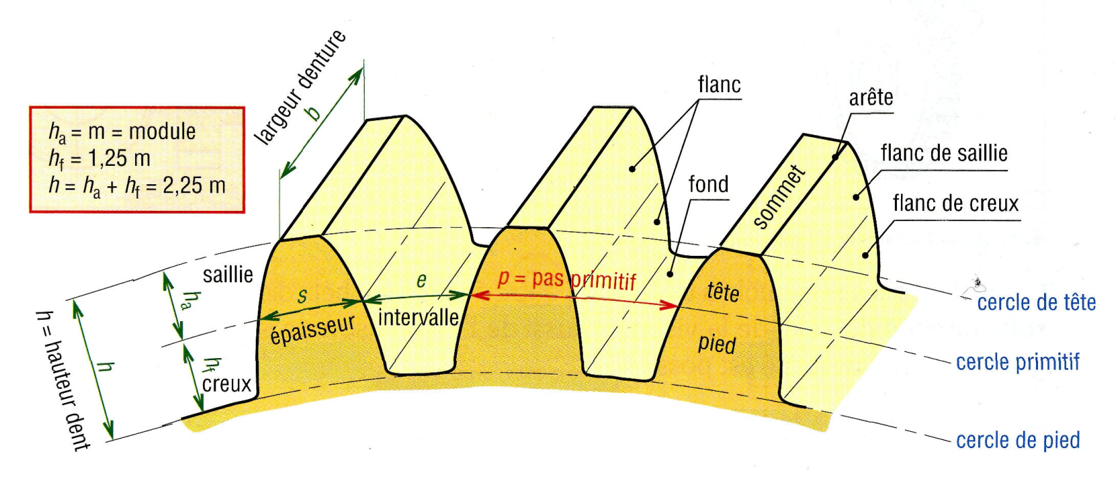
\includegraphics[width=\textwidth]{images/carac_engre}
  \caption{Schéma et caractéristiques d'une roue à denture droite}
  \label{fig:droite}
\end{figure}

\begin{aretenir}~\\
  \begin{itemize}
    \item Une roue droite comporte \trou{un nombre entier de dents}, noté $Z$, placées à intervalles successifs égaux.
    \item La taille de ces intervalles définit le pas $p$ de l'engrenage.
  \end{itemize}
\end{aretenir}

\begin{definition}
  Un engrenage est dit « droit » lorsque les axes de rotation des 2 roues sont parallèles (perpendiculaires à leur plan médiant)
\end{definition}

\subsubsection{Engrenage droit à contact extérieur}
Dans un engrenage à contact extérieur, la denture de chaque roue est sur l’extérieur et le contact se fait par l’extérieur.
Ce sont les plus simples et les plus économiques des engrenages. Toute foi, leur fonctionnement induit des chocs d’engrènement, ce qui provoque du bruit et des vibrations. Ces défauts peuvent être atténués en réduisant le module des engrenages, mais cela diminue aussi leur résistance.
\begin{aretenir}
Un engrenage droit à deux roues est défini par :
\begin{itemize}
  \item Une roue menante (généralement relié à l'arbre du moteur)
  \item Une roue menée qui est entrainée par la roue menante
\end{itemize}
\end{aretenir}

\begin{definition}
  Le rapport $r$, aussi appelé \textit{raison de l'engrenage} est égal à $$r = \frac{Z_{\text{menante}}}{Z_{\text{menante}}} = \frac{\omega_s}{\omega_e}$$

  Avec $Z$ le nombre de dents des roues menante et menée et $\omega_s$ et $\omega_e$ les vitesse d'entrée et de sortie, respectivement.
\end{definition}

\begin{description}
  \item [Si $r<1$] \trou{$r$ est un rapport de réduction car la vitesse de sortie est plus faible que la vitesse d'entrée}
  \item [Si $r>1$] \trou{$r$ est un rapport de transmission. La vitesse de sortie est plus forte que la vitesse d'entrée. }
  \item [Si $r=1$] \trou{La vitesse en entrée est égale à la vitesse en sortie}
\end{description}

\begin{figure}[h]
  \centering
  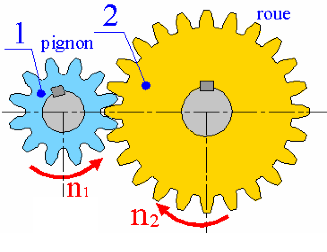
\includegraphics[width=.4\textwidth]{images/engrenage_2_droit}
  \caption{}
  \label{}
\end{figure}

\begin{resultat}~
  \vspace{4cm}
\end{resultat}

\subsubsection{Engrenage droit à contact interieur}
\begin{figure}[h]
  \centering
  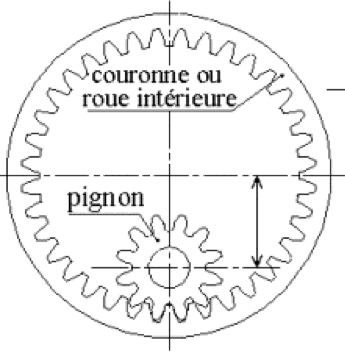
\includegraphics[width=.3\textwidth]{images/engre_interieur}
  \caption{Engrenage à contact intérieur}
  \label{}
\end{figure}
\begin{aretenir}
  \trou{Le fait que le contact se fasse par l’intérieur n’inverse pas le sens de rotation entre les deux roues.}
\end{aretenir}

\subsubsection{Engrenage droit à contact interieur}
Comme les engrenages à denture droite, ils transmettent le mouvement de rotation et la puissance entre deux arbres parallèles, mais leurs dents sont inclinées.
Cette configuration est plus performante et offre une plus grande progressivité et continuité d’engrènement, qui permet de transmettre plus de couple, tout en étant plus silencieux. Ils sont cependant plus complexes à fabriquer.
La transmission des efforts est plus importante (nombres de dents en contacts plus élevés), y compris aux vitesses élevées.
De plus, l’inclinaison des dents induit des efforts latéraux que doivent supporter les paliers de l’engrenage.
Ce type d’engrenage est utilisé dans la transmission des voitures.
\begin{warn}
  Les caractéristiques définies pour les engrenages à contact extérieurs restent valables pour ce type d’engrenage.
\end{warn}

\subsubsection{Engrenages coniques}
  \begin{figure}[h]
    \centering
    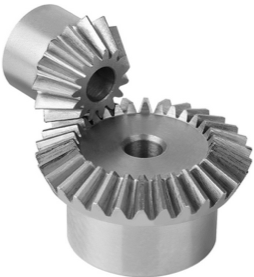
\includegraphics[width=.3\textwidth]{images/engre_conique}
    \caption{Engrenage conique}
    \label{}
  \end{figure}

\begin{definition}
  Un engrenage est dit « conique » lorsque les axes de rotation autour duquel les roues tournent sont sécants
\end{definition}

\subsection{Train d'engrenage}
\begin{definition}
  \trou{Lorsqu’un système mécanique de transmission est composé de plus de deux roues dentées il est appelé train d’engrenage}
\end{definition}

\begin{figure}[h]
  \centering
  \begin{subfigure}{.5\textwidth}
    \centering
    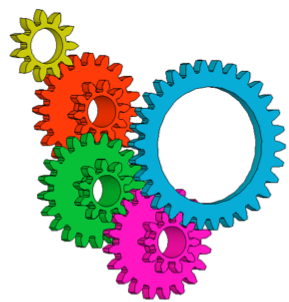
\includegraphics[width=0.9\textwidth,height=.1\textheight,keepaspectratio]{images/train_schema}
    \caption{Schéma d'un train d'engrenage}
  \end{subfigure}\hfill
  \begin{subfigure}{0.5\textwidth}
    \centering
    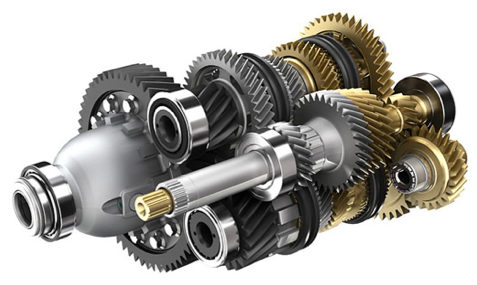
\includegraphics[width=0.9\textwidth,height=.1\textheight,keepaspectratio]{images/train_image}
    \caption{exemple de train d'engrenage}
  \end{subfigure}
\end{figure}
\pagebreak
\begin{aretenir}~
  \vspace{3cm}
\end{aretenir}

\begin{warn}
\begin{description}
  \item [Si n est pair] \trou{Le sens de rotation en sortie est le même que celui en entrée}
  \item [Si n est impair] \trou{Le sens de rotation en sortie est inversé par rapport à celui de l'entrée}
\end{description}
\end{warn}

\section{Transmission par poulie-courroie}
\begin{figure}[h]
  \centering
  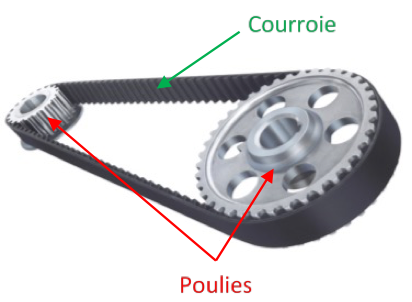
\includegraphics[width=.4\textwidth]{images/poulie-courroie}

  \caption{Système poulie-courroie}
  \label{}
\end{figure}
Ce système permet de transmettre par adhérence, à l’aide d’un lien flexible « la courroie », un mouvement de rotation continu entre deux arbres éloignés.


\begin{aretenir}
  \vspace{4cm}
\end{aretenir}

\begin{warn}
  Le sens de rotation de la poulie réceptrice est le même que celui de la poulie motrice. Pour inverser le sens de rotation, il faut croiser la courroie.
\end{warn}

\end{document}
